\chapter{向量组与线性空间}

\section{Overview}
\begin{figure}[h]
	\centering
	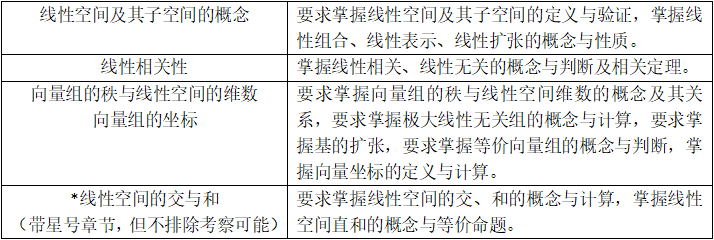
\includegraphics[scale=0.58]{1.png}
\end{figure}

\section{线性空间及其子空间的概念}
\subsection{线性空间的定义}
线性空间是我们接触的第一个比较重要的概念,它是定义在非空集合$V$和数域$\mathbf{F}$
上的,并且定义了$V$中的加法和$V\times \mathbf{F}$(即数域中的数与集合中向量之间的)数乘运算。
总结起来就是非空集合+数域+运算构成的。并且运算满足以下性质:

加法构成交换群$\langle V:+\rangle$(阿贝尔群,见教材1.10节,考试一般不要求)

1. 结合律:$a+(b+c)=(a+b)+c$;

2. 加法单位元:$\exists 0 \in V$,使得$\forall\alpha\in V$,有$a+0=0+a$;

3. 逆元:$\forall\alpha\in V,\exists b\in V$,有$a+b=b+a=0$,记$b=-a$;

4. 交换律:$\forall\alpha,\beta\in V, \alpha+\beta=\beta+\alpha$.

注意:加法零元和逆元是唯一的,我们可以定义减法运算为加上一个元素的逆。

数乘运算也满足四条性质:$\forall \alpha,\beta \in V,\forall \lambda,\mu\in\mathbf{F}$以及$\mathbf{F}$
上的乘法单位元1,有:

1. $1\cdot \alpha=\alpha$;

2. $\lambda(\mu\alpha)=(\lambda\mu)\alpha$;

3. $(\lambda+\mu)\alpha=\lambda\alpha+\mu\alpha$;

4. $\lambda(\alpha+\beta)=\lambda\alpha+\lambda\beta$.

注意,综合上述性质我们有方程$\lambda\beta+\lambda_1\alpha_1+\lambda_2\alpha_2+\cdots+\lambda_r\alpha_r=0$
在$\lambda\neq 0$时的解为$\beta=-\lambda^{-1}\lambda_1\alpha_1+-\lambda^{-1}\lambda_2\alpha_2+\cdots+-\lambda^{-1}\lambda_r\alpha_r$.

以上定义请务必牢记于心,考试可能要求你验证线性空间。记忆难度也并不大,阿贝尔群四条性质都有名称标注,
数乘运算也是结合律和分配律加单位元。

注意线性空间还有一个重要的概念是运算封闭,即线性空间中的元素进行加法或数乘运算后,得到的元素仍然是属于线性空间的。
这一点是定义要求的,加法封闭是阿贝尔群的要求,数乘请参考教材定义的要求。
\subsection{线性空间举例}
我们介绍三个常见的线性空间:

1. (多项式)$\mathbf{F}[x]_{n+1}=\{a_0+a_1x+\cdots+a_nx^n\ |\ a_i\in\mathbf{F}\}$构成线性空间,但
$$\mathbf{F}[x]_{n+1}=\{a_0+a_1x+\cdots+a_nx^n\ |\ a_i\in\mathbf{F},a_i\neq 0\}$$
不构成线性空间。

注:书上常将多项式记为$\mathbf{F}[x]_{n+1}$,表示次数不超过$n$的多项式的集合。

常见记号:$(k_1p_1+k_2p_2)(x)=k_1p_x(x)+k_2p_2(x)$。

2. (复数与实数)可以验证:全体复数构成的集合是数域$\mathbf{C}/\mathbf{R}$上的线性空间。此处一定注意复数$\mathbf{C}$在此处同时出现在集合和数域中。

注意:这一例子表明,同一集合可以在不同数域上构成不同的线性空间。特别是可以验证,线性空间$\mathbf{C(C)}$维数为1,不同于线性空间$\mathbf{C(R)}$维数为2。

当然,不同的集合也可以在同一个数域上构成不同的线性空间,例如$\mathbf{C(R)}$和$\mathbf{R(R)}$。

3. (线性方程组的解)可以验证,齐次线性方程组$AX=0$的解集是线性空间$\mathbf{F^n}$的一个子空间,但非齐次线性方程组的解不再构成线性空间,因为加法运算不封闭。(具体见教材P62的2.2节开头的例子以及P86习题3(3))。
\subsection{线性子空间}
我们首先看线性子空间的定义:
\begin{definition}
	设$W$是线性空间$V(\mathbf{F})$的非空子集,如果$W$对$V$中的运算也构成域$\mathbf{F}$
	上的线性空间,则称$W$是$V$的线性子空间(简称子空间).
\end{definition}
请一定注意定义中的非空子集,建议验证子空间时先验证非空。接下来是验证子空间的一般方法:
\begin{theorem}
	线性空间$V(\mathbf{F})$的非空子集$W$为$V$的子空间的充分必要条件是$W$对于$V(\mathbf{F})$的线性运算封闭.
\end{theorem}
这表明只要子空间中的元素满足对原空间的加法和数乘运算封闭即可。

注意线性空间有两个子空间称为平凡子空间,即仅含零元的子集$\{0\}$和其自身$V$。其它
子空间称为非平凡子空间。
\begin{example}
	\textup{(1)}说明$\mathbf{R}[x]_2$是$\mathbf{R}[x]_3$的子空间\textup{;}

	\textup{(2)}判断$W_1=\{(x,y,z)\ |\ \cfrac{x}{3}=\cfrac{y}{2}=z\},
	W_2=\{(x,,y,z)\ |\ x+y+z=1,x-y+z=1\}$是否为$\mathbf{R}^3$的子空间.
\end{example}
第二小问表明过原点的直线/平面构成三维空间的子空间,不过原点的无法保持线性性。

接下来我们讨论线性扩张及其性质,我们首先来看线性组合和线性表示的概念:
\begin{definition}
	设$V(\mathbf{F})$是一个线性空间,$\alpha_i\in V,\lambda_i\in \mathbf{F}(i=1,2,\cdots,m)$,
	则向量$\alpha=\lambda_1\alpha_1+\lambda_2\alpha_2+\cdots+\lambda_m\alpha_m$
	称为向量组$\{\alpha_1,\alpha_2,\cdots,\alpha_m\}$在域$\mathbf{F}$的线性组合,或说$\alpha$
	在域$\mathbf{F}$上可用向量组$\{\alpha_1,\alpha_2,\cdots,\alpha_m\}$线性表示.
\end{definition}
基于此,我们给出线性扩张的定义:
\begin{definition}
	设$S$是线性空间$V(\mathbf{F})$的非空子集,我们称
	$$L(S)=\{\lambda_1\alpha_1+\cdots+\lambda_k\alpha_k\ |\ \lambda_1,\cdots,\lambda_k\in\mathbf{F},\alpha_1,\cdots,\alpha_k\in S,k\in\mathbf{N^*}\}$$
	为$S$的线性扩张,即$S$中所有有限子集在域$\mathbf{F}$上的一切线性组合组成的$V(\mathbf{F})$的子集.
\end{definition}
下面的定理告诉我们可以通过线性扩张构造子空间:
\begin{theorem}
	线性空间$V(\mathbf{F})$的非空子集$S$的线性扩张$L(S)$是$V$中包含$S$的最小子空间.
\end{theorem}
这一定理的证明首先证明线性扩张是子空间,这是容易的,然后说明最小只需要说明$L(S)$是$V$中包含$S$的任意子空间的子集即可。

最后我们再说明有限维线性空间和无限维线性空间的定义,本课程研究的内容都在有限维线性空间:
\begin{definition}
	$V(\mathbf{F})$称为有限维线性空间,如果$V$中存在一个有限子集$S$使得$L(S)=V$,反之称为无限维线性空间.
\end{definition}
\begin{example}
	证明:$\mathbf{R}[x]_3$是有限维线性空间,$\mathbf{R}[x]$是无限维线性空间.
\end{example}
\subsection{习题}
\centerline{\heiti A组}
\begin{enumerate}
	\item 检验下列集合对指定的加法和数乘运算是否构成实数域上的线性空间.
	
	(1)有理数集$\mathbf{Q}$对普通的数的加法和乘法;

	(2)集合$\mathbf{R}^2$对通常的向量加法和如下定义的数量乘法:$\lambda\cdot(x,y)=(\lambda x,y)$;

	(3)$\mathbf{R}_+^n$(即$n$元正实数向量)对如下定义的加法和数乘运算:
	$$(a_1,\cdots,a_n)+(b_1,\cdots,b_n)=(a_1b_1,\cdots,a_nb_n),$$
	$$\lambda\cdot(a_1,\cdots,a_n)=(a_1^\lambda,\cdots,a_n^\lambda).$$

	(4)请继续完成教材P86第二章习题第一题9-11小问关于函数的加法数乘定义线性空间的问题.
	\item 请完成教材P86-86第二章习题第三题的全部小问.第5小问平常问题较多,实际上就是要判断满足一定条件的
	多项式是否构成子空间.
\end{enumerate}
\centerline{\heiti B组}
\begin{enumerate}
	\item 设$V$是一个线性空间,$W$是$V$的子集,证明:$W$是$V$的子空间$\iff L(W)=W$.
	\item 回答以下两个问题:

	(1)设$\mathbf{R}^+$是所有正实数组成的集合,加法和数乘定义如下:$\forall a,b \in \mathbf{R}^+,k\in \mathbf{R},a\oplus b = ab, k\odot a = a^k$,$\mathbf{R}^+$关于这一加法和数乘构成一个实线性空间,求$\mathbf{R}^+$的一组基;

	(2)设$V$是一个$n$维实线性空间,证明:存在$V$中的一个由可列无穷多个向量组成的向量组$\{\alpha_i\ |\ i\in\mathbf{Z}^+\}$,使得其中任意$n$个向量组成的向量组都是$V$的一组基.
\end{enumerate}
\centerline{\heiti C组}
\begin{enumerate}
	\item 设$E$是域$F$的一个子域.
	
	(1)证明:$F$关于自身的加法和乘法构成一个$E$上的向量空间,并举一例;

	(2)举例说明:$E(E\neq F)$不是$F$上的线性空间;

	(3)证明:若$V$是$F$上的一个线性空间,则$V$也是$E$上的一个线性空间.
\end{enumerate}

\section{线性相关性}
\subsection{线性相关性的定义}
研究线性相关性来源于我们希望知道有限维线性空间至少需要多少个向量张成,以下是其定义:
\begin{definition}
	设$V(\mathbf{F})$是一个线性空间,$\alpha_1,\alpha_2,\cdots,\alpha_m\in V$,如果存在
	不全为$0$的$\lambda_1,\lambda_2,\cdots,\lambda_m\in\mathbf{F}$,使得
	$$\lambda_1\alpha_1+\alpha_2\lambda_2+\cdots+\lambda_m\alpha_m=0$$
	成立,则称$\alpha_1,\alpha_2,\cdots,\alpha_m$线性相关,否则称线性无关(即系数只能为$0$).
\end{definition}
线性相关和线性无关的证明就是基于这个定义,请务必牢牢掌握。

直接由定义我们可以导出以下结论:

1. 线性空间中单个向量$\alpha$线性相关的充要条件是$\alpha$为零向量;

2. 任何含零向量的向量组都线性相关.

我们来看几个基本的例子:
\begin{example}
	\textup{(1)}判断$(1,1,0),(0,1,1),(1,0,-1)$的线性相关性;

	\textup{(2)}判断$(1,-3,1),(-1,2,-2),(1,1,3)$的线性相关性;

	\textup{(3)}判断$p_1(x)=1+x,p_2(x)=1-x,p_3(x)=x+x^2$的线性相关性;

	\textup{(4)}判断$1,\sin^2x,\cos^2x$的线性相关性;

	\textup{(5)}判断$1,2^x,2^{-x}$的线性相关性.
\end{example}
注意上述3-5题为不能代入特殊的$x$值来说明,例如(3)令$x=0$得到线性相关的做法是错误的,因为
(3)中线性空间就是多项式构成的线性空间,其中的元素就是多项式,不能代入值。注意(5)是特殊题型,
需要构造更多的方程来求解这一问题。
\subsection{线性相关性的定理}
本节内容十分重要,是理解线性空间结构的基础,希望同学们对以下定理及其证明十分熟练并且要有深刻的理解。
我们的主线思路是从不同方面理解线性相关性:
\begin{enumerate}
	\item 从线性组合看(定义)
	
	向量组线性相关$\iff$它们有系数不全为0的线性组合等于零向量;
	
	向量组线性无关$\iff$它们只有系数全为0的线性组合才会等于零向量。
	\item 从线性表示看(教材定理2.3)
	\begin{theorem}
		线性空间$V(\mathbf{F})$中的向量组$\alpha_1,\alpha_2,\cdots,\alpha_m(m \ge 2)$线性相关的充分必要条件是
		$\alpha_1,\alpha_2,\cdots,\alpha_m$中有一个向量可由其余向量在域$\mathbf{F}$上线性表示.
	\end{theorem}
	这一定理等价描述为,向量组线性无关的充分必要条件是其中的向量无法互相表示。这是显然的,因为向量组能互相表示
	利用定义可以轻松写出非零系数的线性表示。总结一下即为:

	向量组线性相关$\iff$其中至少有一个向量可以由其余向量线性表示;
	
	向量组线性无关$\iff$其中每一个向量都不能由其余向量线性表出。
	\item 从齐次线性方程组看(教材P66例3,实际上这一点与定义十分类似)

	列向量组$\alpha_1,\alpha_2,\cdots,\alpha_m$线性相关$\iff$齐次线性方程组$x_1\alpha_1+x_2\alpha_2+\cdots+x_m\alpha_m=0$有非零解;

	列向量组$\alpha_1,\alpha_2,\cdots,\alpha_m$线性无关$\iff$齐次线性方程组$x_1\alpha_1+x_2\alpha_2+\cdots+x_m\alpha_m=0$只有零解。
	\item 从向量组线性表示一个向量的方式看(教材定理2.4)
	\begin{theorem}
		若向量组$\alpha_1,\alpha_2,\cdots,\alpha_m$线性无关,而向量组$\beta,\alpha_1,\alpha_2,\cdots,\alpha_m$线性相关,
		则$\beta$可由$\alpha_1,\alpha_2,\cdots,\alpha_m$线性表示,且表示法唯一.
	\end{theorem}
	总结如下:若向量组外另一向量可由这一组向量线性表示,则

	向量组线性无关$\iff$表出方式唯一;

	向量组线性相关$\iff$表示方式有无穷多种。

	表示方式唯一的证明是经典的,即设有另一种表示方式,然后利用线性无关的定义说明这两种表示方式必定相同即可。
	\item 从向量组与它的部分组的关系看(教材P67例6)
	
	如果向量组的一个部分组线性相关,那么整个向量组也线性相关;

	如果向量组线性无关,那么它的任何一个部分组也线性无关。
\end{enumerate}
除此之外,我们还可以从矩阵的秩以及行列式是否为0的角度理解,这些内容后续会有介绍。

最后我们还要介绍一个定理,这一定理更加重要,证明可能较为复杂,但结论一定要熟练掌握:
\begin{theorem}
	设$V(\mathbf{F})$中向量组$\{\beta_1,\beta_2,\cdots,\beta_s\}$的每个向量可由另一向量组$\alpha_1,\alpha_2,\cdots,\alpha_r$
	线性表示.若$s>r$,则$\{\beta_1,\beta_2,\cdots,\beta_s\}$线性相关.
\end{theorem}
这一定理的等价命题为,$\{\beta_1,\beta_2,\cdots,\beta_s\}$线性无关则必有$s\le r$。

这一定理可通俗概括为:多的向量组可以被少的向量组线性表示,多的一定线性相关。反过来说,线性无关的向量只能被等长或更长的向量组线性表示。
\subsection{习题}
\centerline{\heiti A组}
\begin{enumerate}
	\item 请先完成教材P87-88第二章习题第10题的判断题;
	\item 证明:如果向量组线性相关,把每个向量去掉$m$个位置一致的分量,得到的缩短组仍线性相关;
	如果向量组线性无关,把每个向量添加$m$个位置一致的分量,得到的缩短组仍线性无关;
	\item $a$取何值时,$\beta_1=(1,3,6,2)^\mathrm{T},\beta_2=(2,1,2,-1)^\mathrm{T},\beta_3=(1,-1,a,-2)^\mathrm{T}$
	线性无关?
	\item 设$\alpha_1,\alpha_2,\cdots,\alpha_n\in\mathbf{F}^n$,证明:$\alpha_1,\alpha_2,\cdots,\alpha_n$线性无关
	的充要条件是$\mathbf{F}^n$中任一向量都可以由它们线性表示.
	\item 设$S_1=\{\alpha_1,\cdots,\alpha_s\},S_2=\{\beta_1,\cdots,\beta_t\}$是向量空间$V$的两个线性无关的子集,证明:
	$\alpha_1,\cdots,\alpha_s,\beta_1,\cdots,\beta_t$线性无关$\iff L(S_1)\cap L(S_2)=\{0\}$.
\end{enumerate}
\centerline{\heiti B组}
\begin{enumerate}
	\item 已知$\alpha_1\neq 0$,则$\alpha_1,\alpha_2,\cdots,\alpha_n$线性相关的充要条件是存在$i(2\le i\le n)$
	使得$\alpha_i$可由$\alpha_1,\alpha_2,\cdots,\alpha_{i-1}$线性表示,且表示法唯一.
	\item 设 $\sigma$ 是线性空间 $V$ 上的线性变换,如果 $\sigma^{k-1}(\alpha) \neq 0$,但 $\sigma^{k}(\alpha) = 0$,证明:\newline
	$\alpha,\ \sigma(\alpha),\ \dots,\ \sigma^{k-1}(\alpha)(k>0)$ 线性无关
	(本题还有对应的矩阵版本,解法基本一致).

	注:以上两题要采用从右向左/从左向右检查第一个不为0的系数的方法,这种思想是重要的.
	\item 设向量组$\alpha_1,\alpha_2,\cdots,\alpha_n$线性无关,在向量组$\beta,\alpha_1,\alpha_2,\cdots,\alpha_n$中至多有一个向量$\alpha_i(1\le i\le r)$
	可被其前面的$i$个向量$\beta,\alpha_1,\alpha_2,\cdots,\alpha_{i-1}$线性表示.
	\item 证明:$1,e^{\lambda_1\cdot x},e^{\lambda_2\cdot  x}(\lambda_1\neq\lambda_2$且均不为0$)$线性无关.
\end{enumerate}
\centerline{\heiti C组}
\begin{enumerate}
	\item 如果$n$阶方阵$A_1,A_2,\cdots,A_m$满足$A_i^2\neq O(i=1,2,\cdots,m)$,且当$i\neq j$时,$A_iA_j=O$,
	证明:$m\le n$.
	\item 已知$m$个向量$\alpha_1,\alpha_2,\cdots,\alpha_m$线性相关,但其中任意$m-1$个都线性无关,证明:
	
	(1)若$k_1\alpha_1+\cdots+k_m\alpha_m=0$,则$k_1,\cdots,k_m$全为0或全不为0;

	(2)若存在两个等式
	$$k_1\alpha_1+\cdots+k_m\alpha_m=0,$$
	$$l_1\alpha_1+\cdots+l_m\alpha_m=0,$$
	其中$l_1\neq 0$,证明:$\cfrac{k_1}{l_1}=\cdots=\cfrac{k_m}{l_m}$.
\end{enumerate}

\section{向量组的秩\ 线性空间的维数\ 向量组的坐标}
\subsection{秩与维数的概念}
\begin{definition}
	若线性空间$V(\mathbf{F})$的非空子集$S$中存在线性无关的向量组$B=\{\alpha_1,\alpha_2,\cdots,\alpha_m\}$,
	且$S$中每个向量都可以由$B$线性表示,则$B$中向量的个数$r$叫做$S$的秩,记作$r(S)= r$(实际上即为极大线性无关组的长度).
\end{definition}
\begin{definition}
	若线性空间$V(\mathbf{F})$的有限子集$B=\{\alpha_1,\alpha_2,\cdots,\alpha_n\}$线性无关,且$L(B) = V$,则称$B$为$V$的一组基,
	并称$n$为$V$的维数,记作$\dim V = n$.
\end{definition}
实际上,综合上述两个定义我们可以看到,如果$S$为有限维线性空间$V(\mathbf{F})$的子空间,那么$S$的秩就是$S$的维数。

从维数的定义中我们可以理解到,一个线性空间的基的长度必定是唯一的,否则同一个线性空间将会出现多个不同的维数,这是不合理的。
证明可以直接利用上一小节中的定理1.3.3,反证法即可。当然我们也可以不利用定理1.3.3,直接通过线性无关的定义以及线性方程组的解的情况讨论
得到线性空间维数唯一的结论(大家可以自行尝试,实际上我的期中复习2021版中也有讲解)。

我们需要提及一个概念,即自然基。例如三维空间的自然基为$(1,0,0),(0,1,0),(0,0,1)$,$n$维空间也有类似的推广(即$n$个只有一位为0其余全为1的向量)。
对于多项式我们则将$1,x,x^2,\cdots$称为自然基,矩阵、函数等也有相关的常用的基。
\subsection{相关定理与性质}
根据秩与维数的概念与定理1.3.3(或教材定理2.5),我们可以得到以下直接的结论:

1. $r(S)=n$,则$S$中$n+1$个向量必线性相关,$S$中任何线性无关向量组至多含$n$个向量,且将含$n$个线性无关向量的
向量组称为$S$的极大线性无关组。同理,$n$维线性空间中$n+1$个向量必线性相关,其中含$n$个线性无关向量的向量组称为
线性空间的一组基;

注意:极大线性无关组有两个关键词:线性无关与张成空间,我们还有两个结论:
\begin{itemize}
	\item 设向量组的秩为$r$,则它的任意$r$个线性无关的向量都构成它的一个极大线性无关组;
	\item 设向量组的秩为$r$,则若向量组可以由其中的$r$个向量线性表出,那么这$r$个向量就是原向量组的一个极大线性无关组。
\end{itemize}

2. 线性空间的基的个数(维数)是唯一的,但基中向量选取不唯一;

3. 若$r(S)=r$,$B=\{\alpha_1,\alpha_2,\cdots,\alpha_r\}$是$S$的极大线性无关组,则$L(S)=L(B)$,
即$\dim L(S)=r(S)$(秩与维数统一).

接下来我们介绍等价向量组的概念。我们称可以互相线性表示的两个向量组为等价向量组。可以回忆教材1.3节等价关系,可知等价向量组必须满足自反性、对称性以及传递性。
这一点是容易证明的。注意,等价向量组必定秩相等,这是由定理1.3.3(教材定理2.5)可以直接导出的。
关于等价向量组,在后续专题过渡矩阵中还有更多的讨论。

实际上上述结论将向量组的线性扩张替换为线性空间,向量组的秩替换为线性空间的维数,向量组的极大线性无关组替换为线性空间的基,
我们能得到大量等价的结论。除此之外还有和线性相关性以及秩有关的很多结论,我们在这两节习题中展示。
\begin{example}
	证明以下两个结论:

	\textup{(1)}设$U$和$W$都是$V$的非零子空间,如果$U\subseteq W$,那么$\dim U \le \dim W$;
	
	\textup{(2)}设$U$和$W$都是$V$的非零子空间,$U\subseteq W$,且$\dim U = \dim W$,则$U = W$.
\end{example}
最后是一个很重要的定理,这一定理在之后大量的定理证明中都有运用:
\begin{theorem}
	如果$W$是$n$维线性空间$V$的一个子空间,则$W$的基可以扩充为$V$的基.
\end{theorem}
这一定理表明我们可以往一个向量组添加向量扩充为基,之前我们通过求极大线性无关组丢掉一些向量
使得我们获得一组基。定理证明是简单的,实际上这就是教材定理2.6。
\subsection{求解极大线性无关组}
我们首先考察一个阶梯矩阵$A$。我们不难发现,阶梯矩阵的主元(非零行的第一个非零元素)所在的列
构成$A$的列向量的一个极大线性无关组。证明可以利用行列式的秩的相关概念,取出矩阵的子式考虑其行列式。

但我们一般的题目不会直接给出能够成阶梯矩阵的向量,但我们知道,矩阵经过初等行变换不改变列之间的
线性关系(思考其证明),所以我们求极大线性无关组的方法就是,将向量按列排列成矩阵,然后对矩阵做
初等行变换,化为阶梯形,找到主元所在的列,对应的原向量即组成一个极大线性无关组。

注意极大线性无关组是不唯一的,但上面给出了一个程式化的方法。实际上如果能一眼看出结果的也不必如此麻烦
(当然题目直接要求极大线性无关组还是应当写具体过程的)。
\begin{example}
	求向量组$\{\alpha_1=(1,-1,2,4),\alpha_2=(0,3,1,2),\alpha_3=(3,0,7,14),\alpha_4=(1,-1,2,0),\alpha_5=(2,1,5,6)\}$
	的极大线性无关组和秩.
\end{example}

\subsection{向量组的坐标}
坐标的概念实际上我们已经熟悉,例如高中学过的平面向量,平面向量的坐标表示就是二维平面的基$(0,1),(1,0)$
下的坐标表示。我们现在将这个概念拓展到更一般的线性空间:
\begin{definition}
	设$B=\{\beta_1,\beta_2,\cdots,\beta_n\}$是$n$维线性空间$V(\mathbf{F})$的一组基,如果$V$中元素$\alpha$
	表示为$\alpha=a_1\beta_1+a_2\beta_2+\cdots+a_n\beta_n$,则其系数组$a_1,a_2,\cdots,a_n$称为$\alpha$在
	基$B$下的坐标,记为$\alpha_B=(a_1,a_2,\cdots,a_n)$.
\end{definition}
我们很容易证明,$(\alpha+\beta)_B=\alpha_B+\beta_B$和$(\lambda\alpha)_B=\lambda\alpha_B$成立,
这表明坐标也保持了原空间的线性运算关系不变。并且我们不难证明坐标与向量是一一对应的,并且坐标处于$\mathbf{F}^n$空间中,
所以我们可以将对一般线性空间的研究转为研究简单的$\mathbf{F}^n$空间,这也是下一章中同构会提及的。

需要注意的是,$\mathbf{R}^n$中的向量在自然基下的坐标实际上就是向量本身,需要牢记。
\begin{example}
	分别求$p(x)=a_0+a_1x+a_2x^2$在基$B_1=\{1,x,x^2\}$和$B_2=\{1,x-1,(x-1)^2\}$下的坐标.
\end{example}
\subsection{习题}
\centerline{\heiti A组}
\begin{enumerate}
	\item 已知$\alpha_1=(1,2,4,3),\alpha_2=(1,-1,-6,6),\alpha_3=(-2,-1,2,-9),\alpha_4=(1,1,-2,7),\beta=(4,2,4,a)$.
	
	(1)求子空间$L(\alpha_1,\alpha_2,\alpha_3,\alpha_4)$的维数和一组基;

	(2)求$a$的值使得$\beta\in W$,并求$\beta$在(1)所选基下的坐标.
	\item 证明:$B=\{1,x-a,(x-a)^2\}(a\neq 0)$是$\mathbf{R}[x]_3$的一组基,并求$\mathbf{R}[x]_3$的
	自然基$\{1,x,x^2\}$中每个向量关于基$B$的坐标.
	\item 已知向量组$A=\{\alpha_1,\alpha_2,\alpha_3\},B=\{\alpha_1,\alpha_2,\alpha_3,\alpha_4\},C=\{\alpha_1,\alpha_2,\alpha_3,\alpha_5\}$
	的秩分别为$r(A)=r(B)=3,r(C)=4$,证明:$\{\alpha_1,\alpha_2,\alpha_3,\alpha_5-\alpha_4\}$的秩为4.
	\item 设向量组$\alpha_1,\alpha_2,\cdots,\alpha_s$的秩为$r$,在其中任取$m$个向量$\alpha_{i1},\alpha_{i2},\cdots,\alpha_{im}$,
	证明:向量组$\alpha_{i1},\alpha_{i2},\cdots,\alpha_{im}$的秩$\ge r+m-s$.
	\item 已知$\alpha_1,\alpha_2,\cdots,\alpha_n$线性无关,且$\alpha_1,\alpha_2,\cdots,\alpha_n,\beta,\gamma$线性相关,
	证明:要么$\beta,\gamma$可以由$\alpha_1,\alpha_2,\cdots,\alpha_n$线性表示,要么$\alpha_1,\alpha_2,\cdots,\alpha_n,\beta$
	与$\alpha_1,\alpha_2,\cdots,\alpha_n,\gamma$等价.
\end{enumerate}
\centerline{\heiti B组}
\begin{enumerate}
	\item 设线性空间$V(\mathbf{F})$中,向量$\beta$是$\alpha_1,\cdots,\alpha_r$的线性组合,但不是$\alpha_1,\cdots,\alpha_{r-1}$的线性组合,
	证明:$L(\alpha_1,\cdots,\alpha_{r-1},\alpha_r)=L(\alpha_1,\cdots,\alpha_{r-1},\beta)$.
	\item 利用列向量线性相关性,证明矩阵秩不等式:$|r(A)-r(B)|\le r(A\pm B) \le r(A)+r(B)$.
	\item $M_n(\mathbb{R})$表示实$n$阶方阵全体构成的集合,设$W=\{A\in M_n(\mathbb{R})\ |\ a_{ji}=ka_{ij},\ i \le j\}$,
	求当$k=0,1,2$时,$W$的一组基和维数.
	\item 设$\mathbf{R}[x]_3$是次数小于3的实系数多项式和全体零多项式一起组成的集合
	关于多项式加法和数乘多项式运算构成的实数域上的线性空间.

	(1)证明:$W=\{f(x)\in \mathbf{R}[x]_3\ |\ f(1)=0\}$是$\mathbf{R}[x]_3$的一个子空间,并求$W$的维数和一组基;

	(2)定义从$\mathbf{R}[x]_3$到$\mathbf{R}$的线性映射$\sigma(f(x))=f(1)$,证明:$\sigma$为线性映射,
	并求$\textup{Im }\sigma$和$\dim\ker\sigma$;

	(3)设$f,g,h \in \mathbf{R}[x]_3$且$f(1)=g(1)=h(1)=0$,证明:$f,g,h$线性相关.
	\item 设$V_1,V_2$是数域$\mathbf{F}$上的线性空间,$\forall (\alpha_1,\alpha_2),(\beta_1,\beta_2)\in V_1\times V_2,\forall k\in\mathbf{F}$,规定
	$$(\alpha_1,\alpha_2)+(\beta_1,\beta_2)=(\alpha_1+\beta_1,\alpha_2+\beta_2),$$
	$$k(\alpha_1,\alpha_2)=(k\alpha_1,k\alpha_2).$$

	(1)证明:$V_1\times V_2$关于以上运算构成数域$\mathbf{F}$上的线性空间;

	(2)若$\dim V_1=m,\dim V_2=n$,求$\dim(V_1\times V_2)$.
	\item (完成本题前可以先回顾专题三矩阵乘法交换问题一节)设$A \in \mathbf{F}^{n \times n}$,令$C(A)=\{B \in \mathbf{F}^{n \times n}\ |\ AB=BA\}$.
	
	(1)证明:$C(A)$为$\mathbf{F}^{n \times n}$的一个子空间;

	(2)当$A=E$时,求$C(A)$;

	(3)当$A$为对角线上元素互不相等的对角阵时,求$C(A)$的维数和一组基.
	\item 设$S(A)=\{B \in \mathbf{F}^{n\times n}\ |\ AB=0\}$.
	
	(1)证明:$S(A)$为$\mathbf{F}^{n\times n}$的子空间;
	
	(2)设$r(A)=r$,求$S(A)$的一组基和维数.
\end{enumerate}
\centerline{\heiti C组}
\begin{enumerate}
	\item (替换定理)设$\alpha_1,\alpha_2,\cdots,\alpha_r$线性无关,且可以被
	$\{\beta_1,\beta_2,\cdots,\beta_n\}$线性表示,则可以从$\{\beta_1,\beta_2,\cdots,\beta_n\}$
	选出$r$个向量替换成$\alpha_1,\alpha_2,\cdots,\alpha_r$后得到与$\{\beta_1,\beta_2,\cdots,\beta_n\}$
	等价的新向量组(注:可以使用数学归纳法证明).
	\item 设线性空间$V=\mathbf{F^n}$,证明:
	
	(1)存在$V$的子空间$W$,使得$W$的任一非零向量的分量均不为0;

	(2)若$V$的子空间$W$的任一非零向量的分量均不为0,则$\dim W=1$;

	(3)若$V$的子空间$W$的任一非零向量的零分量个数均不超过$r$,则$\dim W \le r+1$.
\end{enumerate}

\section{线性空间的交与和}
\subsection{线性空间的交与和的概念}
\begin{definition}
	设$W_1,W_2$是线性空间$V(\mathbf{F})$的两个子空间,则
	$$W_1 \cap W_2=\{\alpha\ |\ \alpha\in W_1 \textup{ and } \alpha\in W_2\};$$
	$$W_1 \cup W_2=\{\alpha\ |\ \alpha\in W_1 \textup{ or } \alpha\in W_2\};$$
	$$W_1 + W_2=\{\alpha_1+\alpha_2\ |\ \alpha_1\in W_1,\alpha_2\in W_2\}$$
	分别称为$W_1$和$W_2$的交、并、和.
\end{definition}
我们要注意,线性空间的交与和仍然是$V$的子空间,请各位同学自行证明。并且$V$的有限个子空间的交与和
仍然是$V$的子空间。

关于线性空间的并,我们必须注意线性空间的并不一定是线性空间,这很容易理解,
因为两个线性空间元素组合在一起,两个线性空间各取一个元素求和显然不一定在并集中,大家
可以自行举反例。我们给出以下结论:
$W_1 \cup W_2$为线性空间$\iff W_1 \subseteq W_2$或$W_2 \subseteq W_1 \iff W_1 \cup W_2=W_1+W_2.$

这一结论证明并不复杂,希望各位同学掌握。$V$的有限个子空间的并仍为$V$的子空间的充要条件是其中有一个
子空间能包含其他所有子空间。

我们可以从几何直观上理解这些概念,例如三维空间中两个不同的过原点的平面构成的线性空间的交是其交线(交线也过原点)构成的线性空间,
其和为整个三维空间。三维空间中一个平面与不在该平面上的直线的交只有零元,和为整个三维空间。
考试时我们遇到反例问题可以首先考虑这些简单的几何图形,当然无法解决时可以考虑$(1,0),(0,1),(1,1)$此类
简单的向量为基构成的空间。

关于线性空间的并我们还有一个重要的覆盖定理:
\begin{theorem}
	设$V_1,V_2,\cdots,V_s$是线性空间$V$的$s$个非平凡子空间,证明:$V$中至少存在一个向量
	不属于$V_1,V_2,\cdots,V_s$中的任何一个,即$V_1 \cup V_2 \cup \cdots \cup V_s\subsetneq V.$
\end{theorem}
这一定理表明,任何一个线性空间都不能被自身有限个非平凡子空间通过并得到。例如,有限条直线的并不可能是一个平面。
定理的证明可以使用数学归纳法,下面是一个应用的例子:
\begin{example}
	设$V_1,V_2,\cdots,V_s$是线性空间$V$的$s$个非平凡子空间,证明:存在$V$的一组基$\alpha_1,\alpha_2,\cdots,\alpha_n$
	都不在$V_1,V_2,\cdots,V_s$中.
\end{example}
\subsection{维数公式}
\begin{theorem}
	设$W_1,W_2$是线性空间$V(\mathbf{F})$的两个子空间,则
	$$\dim W_1+\dim W_2=\dim(W_1+W_2)+\dim(W_1\cap W_2).$$
\end{theorem}
上式称为子空间的维数公式,区别于下一专题中的线性映射基本定理的维数公式。这一定理的证明思想
是重要的,利用基的扩张等技巧,需要同学们熟练掌握,下面是一个证明思想类似的例子:
\begin{example}
	已知$A,B$分别是数域$\mathbf{F}$上的$s \times k$和$k \times n$矩阵,$X$是$n \times 1$
	的列向量,证明:所有满足$ABX=0$的$BX$构成一个线性空间$V$,且维数为$r(B)-r(AB).$
\end{example}
\subsection{直和的概念与等价条件}
我们证明或者和空间很多时候都是利用和空间定义进行向量分解,这种分解唯一时即为直和。我们有如下定义:
\begin{definition}
	设$W_1,W_2$是线性空间$V(\mathbf{F})$的两个子空间,若$W_1 \cap W_2=\{0\}$,则$W_1+W_2$叫做
	$W_1$与$W_2$的直和,记作$W_1\oplus W_2$.此时称$W_1,W_2$为互补子空间,或$W_1$是$W_2$的补空间,
	或$W_2$是$W_1$的补空间.
\end{definition}
我们需要注意,一个线性子空间的补空间并不唯一,请同学们给出相应的例子。

直和有以下等价的命题,我们证明或者利用直和都可以任意选择:
\begin{theorem}
	对子空间$W_1,W_2$,下列命题等价:

	\textup{(1)}$W_1+W_2$是直和,即$W_1 \cap W_2=\{0\}$;

	\textup{(2)}$W_1+W_2$中的每个向量$\alpha$的分解式$\alpha=\alpha_1+\alpha_2(\alpha_1\in W_1,\alpha_2\in W_2)$唯一;

	\textup{(3)}零向量的分解式$0=\alpha_1+\alpha_2(\alpha_1\in W_1,\alpha_2\in W_2)$仅当$\alpha_1=\alpha_2=0$时成立;

	\textup{(4)}$\dim (W_1+W_2)=\dim W_1+\dim W_2$.
\end{theorem}
我们也可以定义有限个子空间的直和,即$V=W_1\oplus+W_2\oplus\cdots\oplus W_n \iff W_i \cap \sum\limits_{j \neq i}W_j=\{0\}$。
等价命题也是上述定理的推广,例如唯一分解、0的分解以及维数公式推广。我们有一个与多空间直和相关的定理:
\begin{theorem}
	若$V=V_1\oplus V_2$,$V_1=V_{11}\oplus\cdots\oplus V_{1s}$,$V_2=V_{21}\oplus\cdots\oplus V_{2t}$,则
	$$V=V_{11}\oplus\cdots\oplus V_{1s}\oplus V_{21}\oplus\cdots\oplus V_{2t}.$$
\end{theorem}
我们证明直和一般有两种思路,一种是先证和,再证直和,我们来看一个例子:
\begin{example}
	数域$\mathbf{F}$上所有$n$级矩阵组成的线性空间$V=M_n(\mathbf{F})$,$V_1$表示所有对称矩阵
	组成的集合,$V_2$表示所有反对称矩阵组成的集合,证明:$V_1,V_2$都是$V$的子空间,且$V=V_1\oplus V_2$.
\end{example}
还有一种证明$V=V_1\oplus V_2$的方式是先令$W=V_1+V_2$,先证明和为直和(即交为$\{0\}$)再证$W=V$即可,
下面是一个例子:
\begin{example}
	设$A$是数域$\mathbf{F}$上的一个$n$阶可逆方阵,$A$的前$r$个行向量组成的矩阵为$B$,后$n-r$个
	行向量组成的矩阵为$C$,$n$元线性方程组$BX=0$与$CX=0$的解空间分别为$V_1,V_2$,证明:$\mathbf{F}^n=V_1\oplus V_2$.
\end{example}
\subsection{习题}
\centerline{\heiti A组}
\begin{enumerate}
	\item 设$V=\{(a_1,a_2,a_3,a_4)\ |\ a_1+a_2+a_3+a_4=0\}$,$W=\{(a_1,a_2,a_3,a_4)\ |\ a_1-a_2-a_3+a_4=0,a_1+a_2+a_3-a_4=0\}$.
	
	(1)证明:$V$和$W$为$\mathbf{R}^4$的子空间;

	(2)分别求$V \cap W$,$V+W$以及$W$的补空间的维数与一组基.
	\item 设 $f_1=-1+x,\ f_2=1-x^2,\ f_3=1-x^3,\ g_1=x-x^2,\ g_2=x+x^3,\ V_1=L\left(f_1,\ f_2,\ f_3\right),\ V_2=L\left(g_1,\ g_2\right)$,求:

	(1)$V_1+V_2$ 的基和维数;

	(2)$V_1 \cap V_2$ 的基和维数;

	(3)$V_2$ 在 $\mathbf{R}[x]_4$ 空间的补。
	\item 在数域$\mathbf{F}$上,已知$V_1,V_2$分别为方程组$x_1+x_2+\cdots+x_n=0$与$x_1=x_2=\cdots=x_n$
	的解空间,求证:$\mathbf{F}^n=V_1\oplus V_2$.
\end{enumerate}
\centerline{\heiti B组}
\begin{enumerate}
	\item 设$$W_1=\left\{\begin{pmatrix}
		x & -x \\ y & z
	\end{pmatrix}\ \bigg|\ x,y,z\in \mathbf{F} \right\},W_2=\left\{\begin{pmatrix}
		a & b \\ -a & c
	\end{pmatrix}\ \bigg|\ a,b,c\in \mathbf{F} \right\}.$$

	(1)证明:$W_1,W_2$是$M_2(\mathbf{F})$的子空间,并求$\dim W_1,\dim W_2,\dim(W_1+W_2),\dim(W_1\cap W_2)$;

	(2)求$W_1\cap W_2$的一组基,并求$A=\begin{pmatrix}
		3 & -3 \\ -3 & 1
	\end{pmatrix}$关于这组基的坐标.
	\item 设$V$是域$\mathbb{F}$上的$n$维线性空间,$\{\alpha_1,\alpha_2,\cdots,\alpha_n\}$
	是$V$的一组基,且
	$$V_1=L(\alpha_1+2\alpha_2+\cdots+n\alpha_n);$$
	$$V_2=\{k_1\alpha_1+k_2\alpha_2+\cdots+k_n\alpha_n\ |\ k_1+\cfrac{k_2}{2}+\cdots+\cfrac{k_n}{n}=0\}.$$
	
	证明:

	(1)$V_2$是$V$的子空间;

	(2)$V=V_1\oplus V_2$.
	\item 设$\mathbf{F}$为数域,$V_1=\{A\in\mathbf{F}^{n\times n}\ |\ A^\mathrm{T}=A\}$,
	$V_2=\{A\in\mathbf{F}^{n\times n}\ |\ A^\mathrm{T}=-A\}$,$V_3=\{A\in\mathbf{F}^{n\times n}\ |\ A$为上三角矩阵$\}$.

	(1)证明:$V_1,V_2,V_3$都是$\mathbf{F}^{n\times n}$的子空间;

	(2)证明:$\mathbf{F}^{n\times n}=V_1+V_3$但不为直和,$\mathbf{F}^{n\times n}=V_2\oplus V_3$.
	\item 已知$V_1,V_2$是有限维线性空间$V$的子空间,且$\dim(V_1+V_2)=\dim(V_1 \cap V_2)+1$,证明:
	要么$V_1 \subseteq V_2$,要么$V_2 \subseteq V_1$.
	\item 证明:和$\sum\limits_{i=1}^{s}V_i$为直和的充要条件是$V_i \cap \sum\limits_{j=1}^{i-1}V_j=\{0\}(i=1,2,\cdots,s)$.
	\item 判断下列说法是否正确:
	
	(1)若$V \subseteq V_1 \cup V_2 \cup \cdots \cup V_s$,则$V=(V_1 \cap V)\cup(V_2 \cap V)\cup\cdots\cup(V_s \cap V)$;

	(2)若$V \subseteq V_1+V_2+\cdots +V_s$,则$V=(V_1 \cap V)+(V_2 \cap V)+\cdots+(V_s \cap V)$.
	\item 设$V$为有限维线性空间,$V_1$为其非零子空间,证明:存在唯一的子空间$V_2$,使得$V=V_1\oplus V_2$的
	充要条件为$V_1=V$.
\end{enumerate}
\centerline{\heiti C组}
\begin{enumerate}
	\item 设$V$是域$\mathbb{F}$上的$n$阶对称矩阵关于矩阵加法和数乘运算构成的线性空间,令
	$$U=\{A\in V\ |\ \textup{tr}(A)=0\},\ W=\{\lambda E\ |\ \lambda\in\mathbf{F}\}.$$

	(1)证明:$U,W$为$V$的子空间;

	(2)分别求$U,W$的一组基和维数;

	(3)证明:$V=U\oplus W$.
	\item 设$W_0,W_1,W_2,\cdots,W_s$是线性空间$V$的$s+1$个非平凡子空间,且$W_0 \subseteq W_1 \cup W_2 \cup \cdots \cup W_s$,
	证明:必存在$i$使得$W_0\subseteq W_i$.
	\item 已知$\sigma_1,\sigma_2,\cdots,\sigma_s$是线性空间$V$上的$s$个两两不同的线性变换,证明:在$V$中
	必存在向量$\alpha$使得$\sigma_1(\alpha),\sigma_2(\alpha),\cdots,\sigma_s(\alpha)$也两两不同.
	\item $A$是数域$\mathbf{F}$上的$n$阶方阵,$f_1(x),f_2(x),\cdots,f_s(x)\in \mathbf{F}[x]$且两两互素,
	且$f(x)=f_1(x)\cdots f_s(x)$,记$n$元齐次线性方程组$f(A)X=0,f_1(A)X=0,\cdots,f_s(A)X=0$的解空间分别为
	$V,V_1,\cdots,V_s$,证明:$V=V_1\oplus\cdots\oplus V_s$.
	
	注:这一题是一个非常重要的结论,我们在特征值专题还能再见到其作用。简单的应用是,
	我们可以直接证明$A^2=A \iff r(A)+r(E-A)=n$,$A^2=E \iff r(A+E)=r(A-E)=n$甚至更高阶的类似的秩等式。
\end{enumerate}